\documentclass[manuscript,anonymous,review]{_acm/acmart}

\AtBeginDocument{%
  \providecommand\BibTeX{{%
    \normalfont B\kern-0.5em{\scshape i\kern-0.25em b}\kern-0.8em\TeX}}}


% Rights management information.
\copyrightyear{2018}
\acmYear{2018}
\setcopyright{acmcopyright}
\acmConference[Conference acronym 'XX]{Make sure to enter the correct conference title from your rights confirmation email}{June 03--05, 2018}{Woodstock, NY}
\acmBooktitle{Woodstock '18: ACM Symposium on Neural Gaze Detection, June 03--05, 2018, Woodstock, NY} 
\acmDOI{0000000.0000000}
\acmISBN{978-1-4503-XXXX-X/18/06}
\acmPrice{15.00}


% Submission ID.
% \acmSubmissionID{123-A56-BU3}


% Switches to the "author year" style for citations and references.
% \citestyle{acmauthoryear}


%%
\begin{document}

%%
\title{The Name of the Title is Hope}

%%
\author{John Appleseed}
\email{john@ucsd.edu}
\orcid{0000-0000-0000-0000}
\affiliation{%
  \institution{University of California San Diego}
  \streetaddress{9500 Gilman Dr}
  \city{La Jolla}
  \state{California}
  \country{USA}
  \postcode{92093}
}

%%
\renewcommand{\shortauthors}{Appleseed, et al.}

%%
% Abstract.
\begin{abstract}
  The abstract should be a brief summary of the paper.
\end{abstract}

%%
% ACM Computing Classification System.
% http://dl.acm.org/ccs.cfm
\begin{CCSXML}
<ccs2012>
  <concept>
    <concept_id>10003120.10003145.10003147.10010923</concept_id>
    <concept_desc>Human-centered computing~Information visualization</concept_desc>
    <concept_significance>500</concept_significance>
  </concept>
  <concept>
    <concept_id>10002951.10003317.10003331</concept_id>
    <concept_desc>Information systems~Users and interactive retrieval</concept_desc>
    <concept_significance>300</concept_significance>
    </concept>
  <concept>
    <concept_id>10011007.10011074.10011099.10011102.10011103</concept_id>
    <concept_desc>Software and its engineering~Software testing and debugging</concept_desc>
    <concept_significance>300</concept_significance>
  </concept>
</ccs2012>
\end{CCSXML}

\ccsdesc[500]{Human-centered computing~Information visualization}
\ccsdesc[300]{Information systems~Users and interactive retrieval}
\ccsdesc[300]{Software and its engineering~Software testing and debugging}

%%
% Keywords.
\keywords{datasets, neural networks, gaze detection, text tagging}


%% Teaser.
\begin{teaserfigure}
  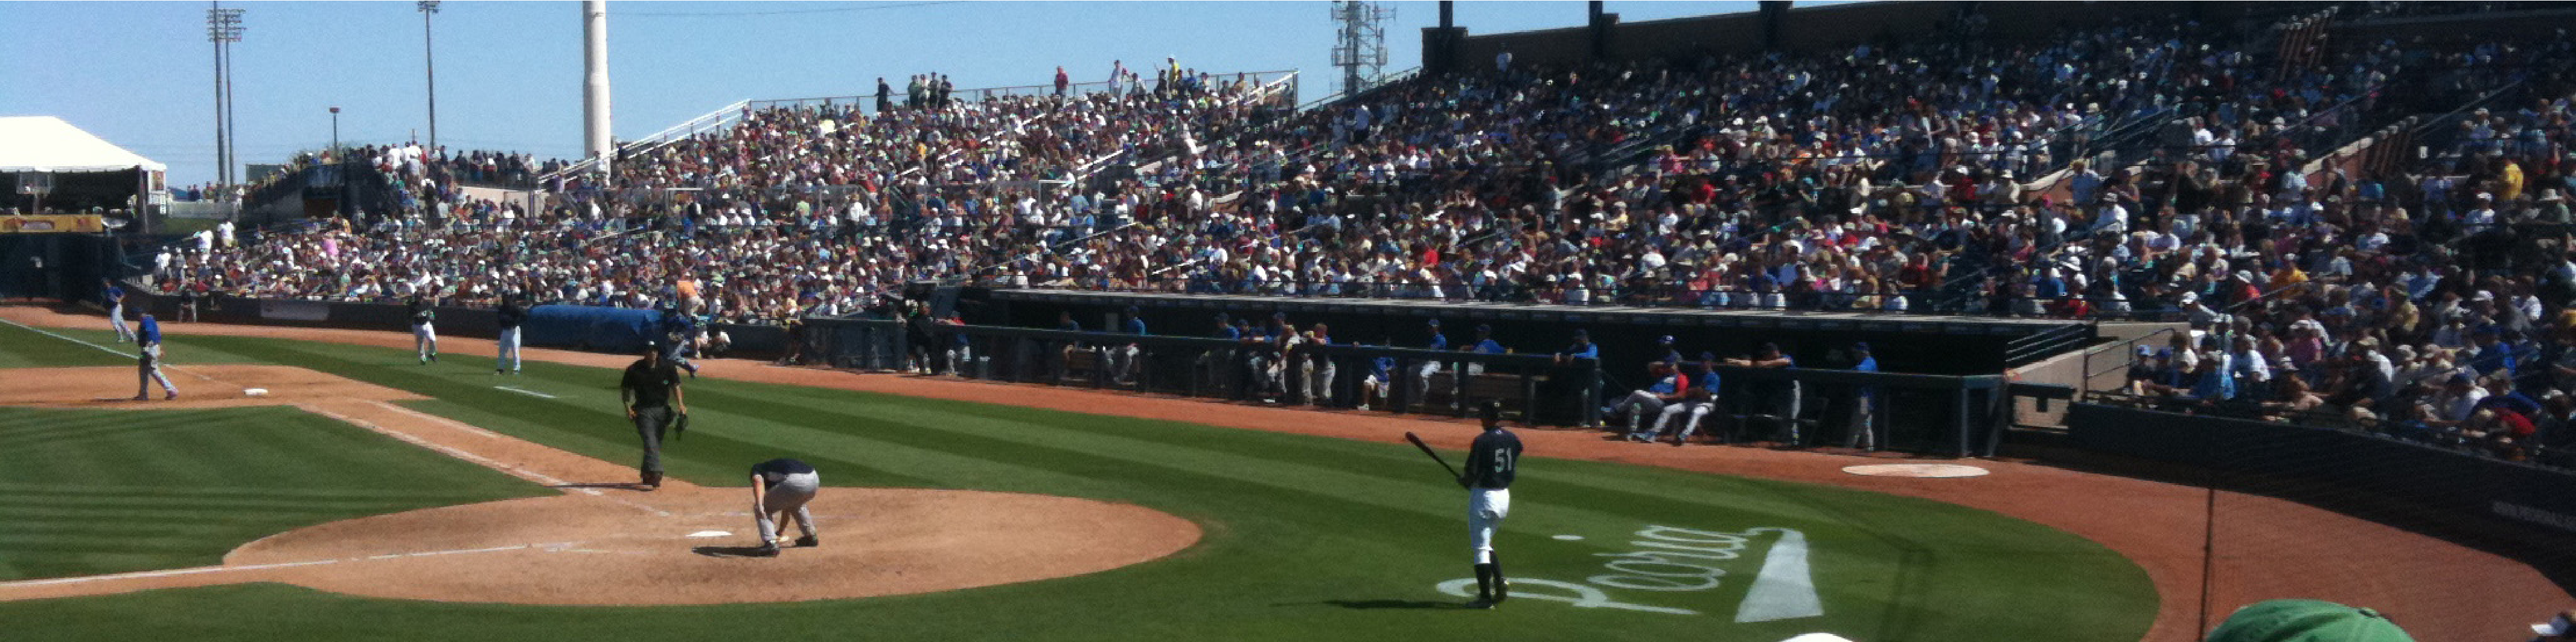
\includegraphics[width=\textwidth]{figures/sampleteaser}
  \caption{Seattle Mariners at Spring Training, 2010.}
  \Description{Enjoying the baseball game from the third-base
  seats. Ichiro Suzuki preparing to bat.}
  \label{fig:teaser}
\end{teaserfigure}


% \received{20 February 2007}
% \received[revised]{12 March 2009}
% \received[accepted]{5 June 2009}


%%
\maketitle


%%
\section{Introduction}
\label{sec:introduction}

The introduction should be a brief summary of the paper.

\section{Related Work}
\label{sec:related}

The present research is based on the prior works~\cite{xia2016object}.

\section{Design}
\label{sec:design}

Introducing the system design.

\section{Evaluation}
\label{sec:evaluation}

Evaluation is an important part of the research process.

\section{Discussion}
\label{sec:discussion}

Discussing the results and the limitations.

\section{Conclusion}
\label{sec:conclusion}

The conclusion should be a brief summary of the paper.



%%
% Acknowledgments.
\begin{acks}
Thanks to the anonymous reviewers for their helpful comments.
\end{acks}


%%
\bibliographystyle{_acm/ACM-Reference-Format}
\bibliography{bibliography}


%%
%% Appendix, this is the place to put it.
% \appendix


\end{document}
\endinput
